\chapter{Artemisa System Architecture}

Once we have a high level architectural view of how an MSX computer works, it is time to start the discussion around how an Artemisa computer implements that architecture.

\section{Features of Artemisa Model 101}

The Artemisa Homebrew DIY model 101 implements most of the parts of the MSX standard have we seen above.

In a few words, Artemisa is an MSX computer with 64KB of RAM memory and two cartridge slots. It has two general purpose (joystick) ports, a data recorder connector, an external keyboard and an interchangeable graphics card. All this encapsulated in a transparent acrylic case of 300x150x35 millimeters.

There are just a few things you typically find in an MSX computer that are not present in Artemisa:

\begin{itemize}
  \item Serial communications port. This can be used to connect modems or other communication devices.
  \item Printer port. Used for printing.
  \item +12- and -12-volts power lines. The built-in hardware of Artemisa use 5 volts power only.
\end{itemize}

However, the +12- and -12-volt lines are included in the pinout of the cartridge connectors. Artemisa wires these pins to ground instead.

\subsection{Keyboard}

Most of the MSX computers, as many other microcomputers built during the 80s, had an integrated keyboard. These computers look like a big keyboard that contains all the elements inside. In contrast, a few MSX vendors followed the same approach as IBM did with their PC: separate the keyboard from the computer connected through a keyboard port. This makes the system less integrated. But also brings some benefits. First, the keyboard can be easily replaced in case of failure. Second, it is easier to manufact computers at scale with different keyboard distributions and layouts, as they only differ in the keyboard.

Artemisa also uses an external keyboard to get advantage from these benefits: reduce the design cost and let the user to choose their keyboard option. It has a custom 25-pin connector that can be used to connect an external keyboard. This can be a custom keyboard built for the Artemisa, or an adapter that allows to connect a PS2 or a USB keyboard.

The Artemisa Homebrew DIY model 101 is shipped by default with a PS2 adapter. You can use it to connect a regular, unexpensive PC keyboard. A microcontroller into the adapter will map the scancodes from the PS2 protocol to simulate a keyboard matrix the MSX will see connected to the port.

\subsection{Graphics card}

The same reasons to have a separated keyboard also applies to have a separated graphics device. Each region has its own TV encoding standards. Some countries use NTSC. Some others use PAL. Some users prefer an unexpensive device that uses composite video output. Some others prefer a RGB output via an SCART connector.

In order to simplify the design and allow the users to customize the video output according to their needs, Artemisa Homebrew DIY separates the graphics card from the rest of the computer motherboard. Both are internally connected using a 50-pin ribbon cable.

\subsection{CMOS Technology}

We will not go too deep in this subject, but it might be worth to discuss a little bit about the semiconductor technologies behind Artemisa.

As you probably know, there was a key invention that boosted the development of computer systems: the transistor. This semiconductor device is the most basic building block used to make basic digital circuits such as logic gates. There are multiple technologies used to implement transistors depending on the semiconductor materials used in the process. Each technology has different properties, constraints and tradeoffs.

During the 70s and 80s, the most used transistor type in consumer electronics was the bipolar junction transistor (BJT). The BJT transistors were the foundations of the Transistor-Transistor Logic technology, or TTL. One of its subfamilies, the TTL-LS, was the de-facto standard used in early microcomputers. The TTL-LS devices switch relatively quick from one logic state to another. This means they have low propagation delays (a voltage change in the input of a gate is quickly reflected in the output voltage), and they can operate at high frequencies (many voltage changes per second can occur). However, this comes in exchange of a high power-consumption. Also, the current they can drive is quite limited. This affects the number of input devices than can be connected to the same output of a TTL device, what is known as the fan-out problem.

In the middle of the 80s, another technology displaced TTL-LS in the consumer electronics market. It was the Complementary Metal-Oxide-Semiconductor (CMOS) technology. It was made up by Metal-Oxide-Semiconductor Field-Effect Transistors (MOSFET). CMOS had two interesting characteristics compared to TTL devices. First, they had a low static power consumption. This means CMOS devices consume much less power than TTL devices when the voltage of their inputs is not changing. Fortunately, for nearly all logic gates in a computer, this is most of the time. This had an interesting side effect: the integration scale is significantly increased. Less power consumption means more transistor density in a chip core (without making the chip burn), what leads to miniaturization. In fact, modern inventions such as the microprocessor were possible thanks to the MOSFET transistors and the derived logic families like NMOS and CMOS. Secondly, CMOS devices can drive more load than TTL equivalents. This practically eliminates the fan-out problem from the equation. These devices also have a better electrical noise reduction. However, the toll paid by CMOS devices is their speed. They respond relatively slow to the changes in their logic state. What cause relatively large propagation delays compared to TTL devices and force them operate at low frequencies. Fortunately, a subfamily known as High-speed CMOS (HCMOS) reduced the propagation delays to acceptable levels.

Roughly speaking, you can assume a TTL logic gate consumes 1000 times the power of its CMOS equivalent. In the other hand, a CMOS device has propagation delays 2x to 5x bigger than their TTL counterparts. The good news is that an MSX computer is a relatively slow machine. The CPU operates at 3.58Mhz and each interaction with the system bus typically involves several clock cycles. The response times are in the range of hundreds of nanoseconds. That is by far in the range of the capabilities of the HCMOS devices.

Taking these considerations, Artemisa uses CMOS devices where possible instead of the TTL equivalents used in the MSX computers designed during the 80s. The glue logic is implemented by integrated circuits of the 74HC family. And the system is designed to operate with Z84C00 and 82C55 chips, the CMOS versions of Z80 microprocessor and the PPI, respectively. There are just a few TTL chips in the design that do not have CMOS equivalents, such as the 74LS07.

\subsection{Integration level}

As discussed in the beginning of this book, Artemisa Homebrew DIY wants to make you learn how an MSX works while you assemble and solder its parts. The easier the assembling process the better. That is why this version of Artemisa sacrifices the miniaturization in favor or an easier soldering experience.

As consequence, all the chips used in the design have Dual Inline Package (DIP) encapsulation.  These are the classic chips used in early microcomputers, formed by two lines of broad pins with a separation of 2.55mm. The same principle is applied to the rest of components. Resistors and capacitors have Through Hole (TH) encapsulation to facilitate the manipulation.

\subsection{Memory technology}

The RAM memory was one of the main limitations of early microcomputers. And not for performance reasons, but costs. Memories were really expensive these days. And engineers had to find ways to make them as affordable as possible.

All RAM memories are made by several x-y matrices of bit cells. For read and write operations, the chip expects to receive the row and column addresses in order to activate the cell where that bit is located and perform the operation. Typically, the bits of the physical memory address are split in two halves such that n less significant bits are the row address and m most significant bits are the column address in the memory matrices. By having eight matrices, one per each bit in a byte, we can implement the system memory of an 8-bit computer.

There are two principal technologies to build RAM devices: DRAM and SRAM. DRAM technology is based on a combination of one capacitor and one transistor to implement each bit cell. The capacitor is used to determine whether the cell contains a logic 1 (charged) or a logic 0 (discharged). The transistor is used as a switch to control the access to the capacitor. Each bit cell is put in a x-y matrix that is addressed by row and column. As it uses only two elements that can be built into a microchip, DRAM is unexpensive compared to other memory technologies.

Unfortunately, DRAM have a big drawback: capacitors tend to discharge by their own. With the time the charge leaks away, so a charged capacitor representing a logic 1 passes to represent a logic 0. Considering the small size of these capacitors, this discharge time is in the order of milliseconds. The RAM chips must refresh the contents of its cells periodically to prevent information lost. In most of the cases, they cannot do that by themselves. And require external circuits to perform the refresh actions periodically. In addition, DRAM chips typically multiplex the pins used for row and column addresses. They depend on a multiplexor circuit to decode the bits from the address bus that belong to row and column. Both the refresh and the row/column multiplexor circuits are not trivial, and they complicate the design of the system.

The alternative to DRAM is the Static RAM (SRAM). This kind of memory uses pure semiconductor devices to implement bistables that can keep 1 bit of information. Typically, six MOSFET transistors are needed per bit cell. What makes them much more expensive than the DRAM equivalents. However, as they do not use capacitors there is no need for refresh circuits.
In the present, the DRAM is still used in modern computers with gigabytes of memory due to its density. SDRAM and DDR technologies are DRAM. However, vendors do not produce DRAM chips for small memory amounts any longer. The SRAM technology has evolved enough to become an unexpensive solution in the range of kilobytes and megabytes. All parts traditionally used in 80s computers are obsolete. And replaces are only available in the secondhand market.

Because of this, and the fact that it simplifies the design of the system, Artemisa uses SRAM memory instead of DRAM. Thanks to this, it does not have to implement a memory refresh circuit or a row/column address multiplexing.

\subsection{Memory layout}

As discussed above, the MSX standard does not define how much memory an MSX computer must have or how it is distributed along the different memory slots.

Artemisa has 64KB of RAM memory located in memory slot 1. These are 4 pages of RAM that occupy the whole slot.

Concerning ROM memory, Artemisa has 32KB of ROM memory where MSX System (MSX BIOS plus MSX Basic) can be found as almost any other MSX system. However, the motherboard provides up to 512KB of total ROM memory. As only 32KB of it are mapped to the MSX in the pages 0 and 1 of memory slot 0, this means the ROM memory has up to 16 different regions of 32KB. Each region contains a different image of the MSX System. A set of 4 jumpers in the motherboard can be used to select the image that will be mapped in the MSX memory space.

The reason to have multiple interchangeable MSX System images is to choose different versions of it, each one supporting different regional configuration. The MSX System image for USA is not the same as the MSX System image for Spain. They expect different keyboard distributions, use a different character set and, in some cases, they even have a different bootscreen message.

\begin{table}[h]
  \centering
  \begin{tabular}{r|l}
    {\bf Jumper config} & {\bf ROM contents}            \\
    {\tt 0b0000}        & MSX System v1.0 International \\
    {\tt 0b0001}        & MSX System v1.0 USA           \\
    {\tt 0b0010}        & MSX System v1.0 Japan         \\
    {\tt 0b0011}        & MSX System v1.0 UK            \\
    {\tt 0b0100}        & MSX System v1.0 France        \\
    {\tt 0b0101}        & MSX System v1.0 Germany       \\
    {\tt 0b0110}        & MSX System v1.0 Italy         \\
    {\tt 0b0111}        & MSX System v1.0 Spain         \\
    {\tt 0b1000}        & MSX System v1.0 Arabic        \\
    {\tt 0b1001}        & MSX System v1.0 Korea         \\
    {\tt 0b1010}        & MSX System v1.0 Russia        \\
    {\tt 0b1011}        & Artemisa Diagnosis Tool v0.1  \\
  \end{tabular}
  \caption{MSX System images stored in the ROM memory}
  \label{table:artemisa-rom-imgs}
\end{table}

The Table \ref{table:artemisa-rom-imgs} summarizes the contents of the Artemisa ROM distribution and the jumper configuration to activate each. As you can see, most of them are MSX System versions. The last one, activated with the jumper configuration 0b1011, is the Artemisa Diagnosis Tool. This is a utility that replaces MSX Basic in order to perform some basic system checks that could be of help diagnosing system problems.

\section{High level architecture}

Now it is time to have a look to the high level architecture of an Artemisa computer. And, what could be better than showing an schematic diagram of the topmost components that comprise the design? This is what you will get from Figure \ref{fig:artemisa-arch-overview}. As you can see, it is likely you are already familiarized to the components shown in that schematic diagram. They are mostly the same elements we have discussed in the previous chapter.

\begin{figure}
  \centering
  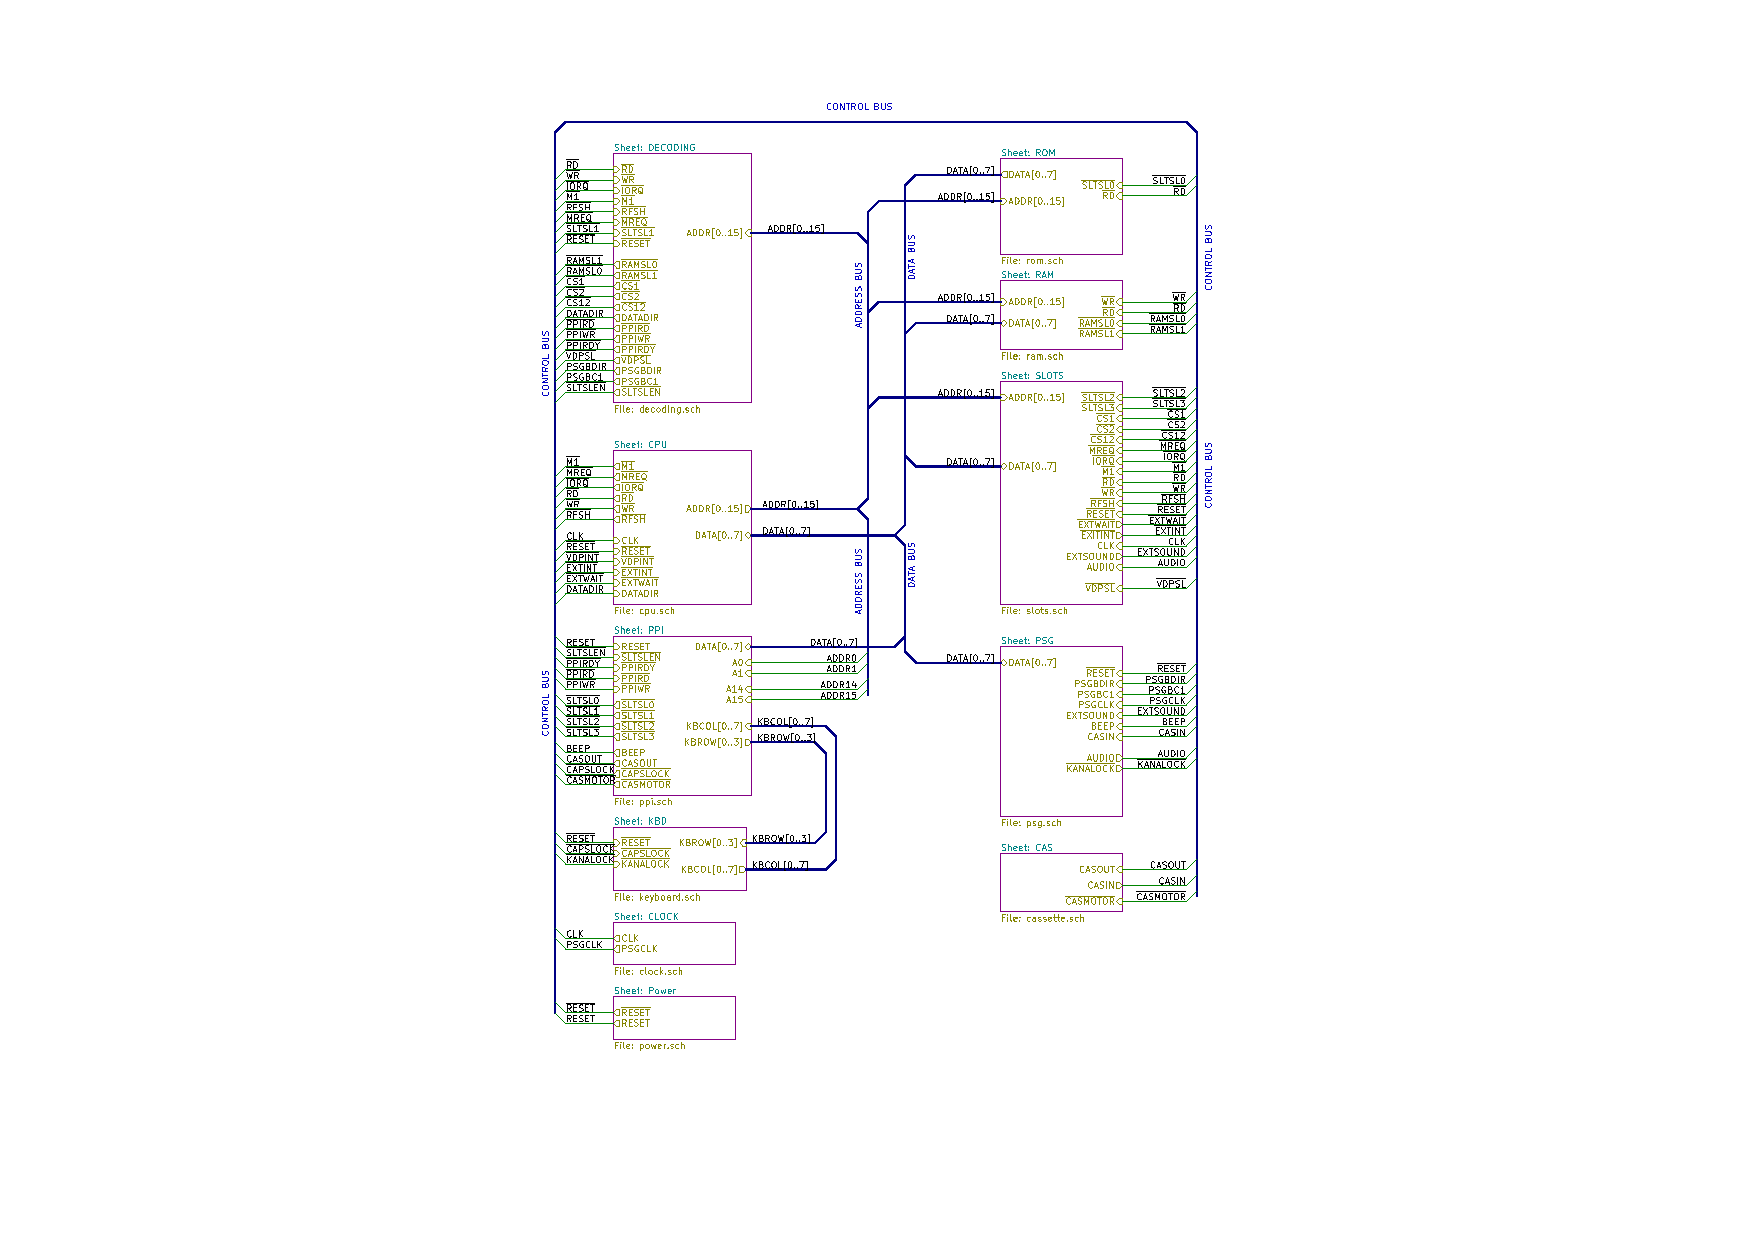
\includegraphics[width=\linewidth,trim={9cm 3cm 9cm 3cm}]{figures/artemisa-schematic-all}
  \caption{High level schematic diagram of an Artemisa MSX Computer}
  \label{fig:artemisa-arch-overview}
\end{figure}

The schematic diagram shows 11 schematic sheets. Each sheet represents a section of the circuit that can be studied separately. You can see the sheets as they were independent integrated circuits or components. In fact, they have pins as any other chip. And the pins are connected to other pins through wires and buses, as in any other schematic diagram. This is what each schematic sheet represents:

\begin{itemize}
  \item {\tt POWER} is the power management sheet. The power connector and the related elements needed to energize the motherboard are described here. The \toref{Power-On Reset} circuit, which is closely related to the power management, is also included here. This is why the outputs of this sheet are mainly the {\tt RESET} and {\tt /RESET} signals.
\end{itemize}

\begin{theory}{Power-On Reset}
  Although this might sound trivial and irrelevant, power-on and reset have a great importance. Once the user presses the power switch on, every component of the system will be energized. They will receive voltage and current from the power supply. But what happens after that?

  Some elements of the system are implemented with something known as {\it sequential logic}. This means they generate their outputs depending not only in their current input signals but also in a sequence of other inputs occurred in the past. They are designed as state machines that will have a different behavior depending on the state they are at each moment. That is the case of the CPU, the VDP, the PSG, the PPI... If we just power on the system, what will be their initial state?

  We can find a good example of sequential logic in the CPU. As you might know, the processor contains an internal register known as the Program Counter (PC). This register indicates the memory address of the next instruction to be fetched. But, what is the value of that register when the CPU is powered on? What will be the first instruction to be executed then?

  The CPU, and any other integrated circuit implemented with sequential logic, provides an input pin where it can receive a signal to be reset into their initial state. This is not only useful when we want to reboot the computer by pressing a reset button, but also when the system is powered up. Receiving electrical current does not mean the state machine will be reset. We have to generate a reset signal when the system is powered up. And... we will see later that this is not as simple as it sounds!
\end{theory}


\begin{itemize}
  \item {\tt CLOCK} is the clock generation circuit. This is a small schematic sheet that will produce squared wave signals of 3.58Mhz and 1.78Mhz used by the Z80 CPU and the AY-3-8910 PSG, respectively.
  \item {\tt CPU} is the sheet where Z80 CPU circuitry is described. This includes all the glue logic to buffer the buses used by the CPU, and the circuit to handle the wait states required by the CPU. If you already know the Z80 CPU pinout, the inputs and outputs of this sheet should be familar.
  \item {\tt DECODING} is the bus decoding logic. This is where the signals from control and address buses are decoded to generate other signals to select actions for other components attached to the buses.
  \item {\tt ROM} is the sheet where the ROM memory is designed.
  \item {\tt RAM} is the sheet where the RAM memory is designed.
  \item {\tt PPI} is the sheet where the Parallel Peripheral Interface is designed. This includes some glue logic necessary to adapt some interfaces.
  \item {\tt PSG} is the sheet where the Programmable Sound Generator is designed. This includes some circuits to adapt the game port interfaces.
  \item {\tt SLOTS} is the sheet where the expansion slots are designed. This includes the connector for the graphics card.
  \item {\tt CAS} is the sheet where the cassette data recorder is designed. This includes the circuits to encode and decode the cassette analog to digital signals.
  \item {\tt KBD} is the sheet where the keyboard interface is designed.
\end{itemize}

Apart from the schematic sheets, we can see in Figure \ref{fig:artemisa-arch-overview} they are also connected among them through a set of buses. These are the control, the address and the data buses we discussed in the previous chapter. But there are also two additional ones: {\tt KBCOL} and {\tt KBROW}. They are the columns and the row address from the keyboard matrix we have also seen before.

As we said in the previous chapter, the design of a 8-bit microcomputer is quite simple. The Figure \ref{fig:artemisa-arch-overview} is all we can find in the motherboard of the Artemisa 101 series. Of course, each schematic sheet contains many elements, so the level of complexity increases as we go deeper in the design. But you do not have to worry. Thanks to having all the elements separated in submodules, we will have the opportunity to cover them separately without feeling overwhelmed.

\section{Anatomy of the Artemisa Model 101}

When all the things are put together into a printed circuit board, the result is as shown in Figure \ref{fig:artemisa-anatomy}.

\begin{figure}[h]
  \centering
  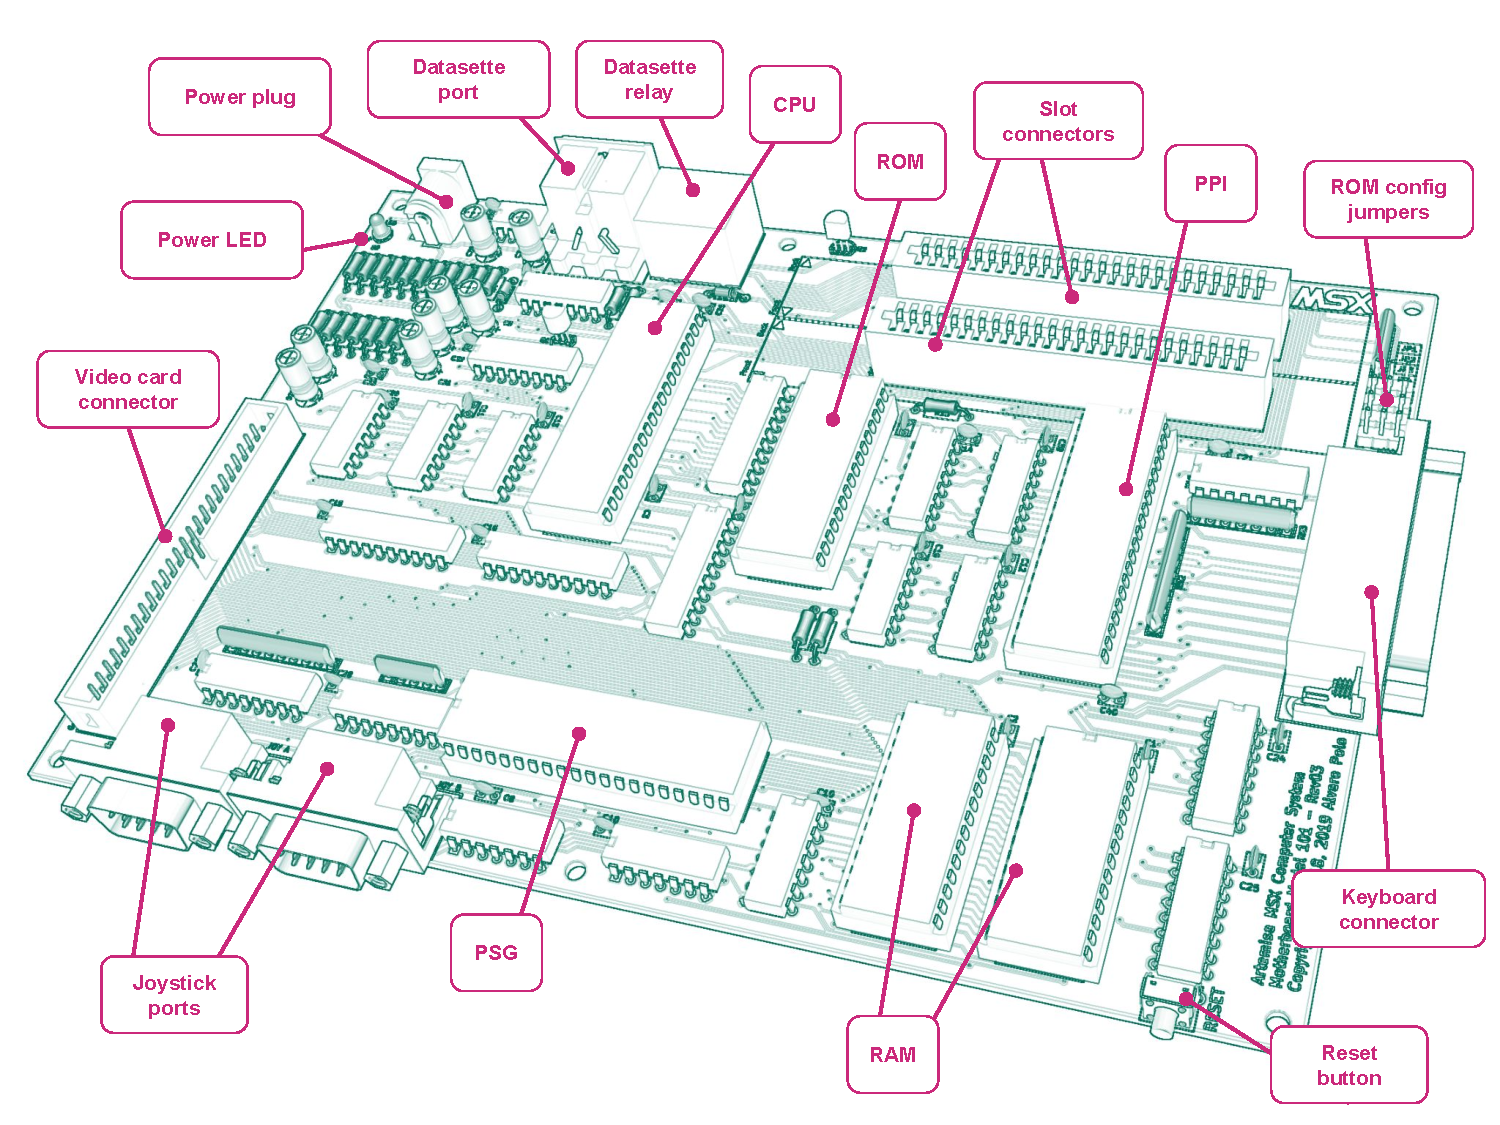
\includegraphics[width=\linewidth]{figures/artemisa-anatomy}
  \caption{Anatomy of the motherboard of an Artemisa computer model 101}
  \label{fig:artemisa-anatomy}
\end{figure}

As you can see, the whole motherboard can be implemented with just 28 integrated circuits, 40 capacitors, 24 resistors, 5 resistor networks, 3 diodes, 2 transistors, 8 connectors, 1 switch, 4 jumpers and 1 crystal oscillator. It will take a few hours to assemble, but its grade of complexity will allow you to understand how an MSX computer works to its most insignificant detail.

It is recommended to observe Figure \ref{fig:artemisa-anatomy} in order to locate the principal components of the motherboard: CPU, RAM and ROM memory, PSG, PPI, etc. But do not bother to memorize it. We will come back to this view when we need it.

Now that you know the high level operation of an Artemisa MSX computer, it is time to prepare for the assembly and discovery process of how it works under the hoods.
